\documentclass[a4paper,12pt]{book}
\usepackage{graphicx} % Required for inserting images
\usepackage{indentfirst}  % Pachet pentru indentarea primei linii
\usepackage{float}
\usepackage{amsmath}

% Pachet pentru caractere românești
\usepackage[utf8]{inputenc}
% Pachet pentru limba română
\usepackage[romanian]{babel}
\usepackage{csquotes}
\bibliographystyle{plain}
\usepackage[nottoc]{tocbibind}
\usepackage{biblatex}

\addbibresource{bibliografie.bib}


% Setări pentru stilul de numerotare a capitolelor
\renewcommand\thechapter{\Roman{chapter}}

% Setări pentru stilul de numerotare a secțiunilor
\renewcommand\thesection{\arabic{section}}

\begin{document}
\frontmatter  % Setează stilul de numerotare pentru partea de început a cărții

\title{SERVICIUL DE GESTIONARE AL REZERVARILOR HORECA}
\author{Cighi Andreea - Maria}
\date{\today}
\maketitle
\tableofcontents  % Generează cuprinsul
\listoffigures
\listoftables

\mainmatter  % Setează stilul de numerotare pentru conținutul principal al cărții

\chapter{Studiu bibliografic}

\indent În acest capitol se vor evidenția conceptele care au stat la baza aplicației, 
cât și referințele teoretice. Totodată, se va efectua o comparație între aplicația propusă și aplicațiile similare existente deja pe piață.

\section{Istoria restaurantelor}
A ieși în oraș pentru a lua masa pare a fi o activitate existentă de când e lumea, dar puțini știu de fapt cum și de ce a apărut această activitate. Marea majoritate a mâncării pe care oamenii o mănâncă acasă în ziua de azi, este fie cea comandată într-un restaurant, fie adusă la ușă de un curier, sau cea gata preparată și achiziționată din supermarketuri, necesitând doar încălzirea ei la microunde pentru a putea fi consumată. Ceea ce ne duce la ideea că mâncatul în casă este mai degrabă o extensie a mâncatului în oraș, când defapt ar trebui să fie exact invers.
Persoanele din ziua de azi doresc din ce în ce mai mult să găsească originile lucrurilor care le trezesc intereseul. De exemplu, le place să știe cum au apărut și au evoluat lucrurile care astăzi pot fi considerate lucruri obișnuite, zilnice. Așa se întâmplă și în cazul istoriei mâncatului. Pentru a elucida acest mister, mâncatul a apărut, după spusele co-autorilor Katie Rawson și Elliott Shore, în urmă cu aproximativ două milioane și jumătate de ani când oamenii din acea vreme au dezvoltat abilități de tăiere și mărunțire, cu scopul de a digera mai ușor mâncarea . Acum 300,000 și 30,000  de ani, agricultura și gătitul a început să ia amploare în rândul oamenilor din acea vreme. \cite{History}
Chiar și în acele vremuri, oamenii își pregăteau mâncarea pentru a avea ce mânca la muncă sau pentru zilele în care aveau de călătorit departe de casă. Totuși, termenul de restaurant era unul necunoscut la acea vreme. Restaurantele cunoscute de ei purtau denumirea de taverne, unde oamenii făceau popas din drumul pe care îl parcurgeau. Meniul sau opțiunea de ați alege singur mâncarea, nu exista în acele timpuri, astfel,  felul de mâncare era întotdeauna la alegerea bucătarului.
Evidența materială a cum a început mâncatul datează din Epoca Cuprului, când oamenii au început să produca vase din ceramică în nordul Mesopotamiei, pentru a putea fi date muncitorilor în schimbul prestărilor de servicii existente în vremea respectivă. Aceste vase au început să fie cu timpul tot mai ornate, variind în mărime, precum se observa si in Figura (\ref{fig:vasOrnat}).

\begin{figure}[htbp]
\centering
  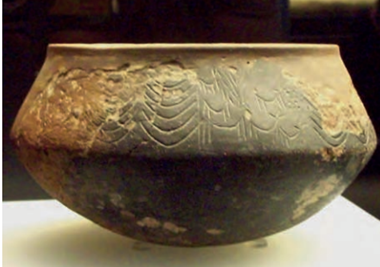
\includegraphics[width=0.5\linewidth]{poza1.png}
  \caption{Vas ornat ce datează din anii 2500-2001 înaintea Erei noastre}
  \label{fig:vasOrnat}
\end{figure}
Confrom studiilor, există dovezi care atestă că oamenii au început să mănânce înafara casei încă din Egiptul antic, datorită ruinelor rămase. În timpurile Romei antice, s-au găsit printre ruinele lui Pompeii, așa zisele termopoluri, locul unde se servea mâncare și băutură diferitelor clase sociale de oameni. Termopolurile erau considerate ca fiind “fast-food-ul” Romei antice. Numele are origini grecești, termopol însemnând defapt “lucruri calde” sau “magazin cald”. Mâncarea era servită în boluri încorporate direct în piatra în formă de “L”. 
Potrivit lui Elliot Shore și Katie Rawson, co-autorii cărții "Dining Out: A Global History of Restaurants", primele clădiri care au fost recunoscute ca fiind restaurante,  datează din jurul anilor 1100 după Hristos, în China, unde orașe precum Kaifeng și Hangzhou și-au crescut numărul populației cu peste un milion de locuitori fiecare.\cite{History}
În lumea antică, oamenii mâncau în general doar cu persoanele pe care le cunoșteau, dar existau totuși ocazii când se aflau la masă și persoane necunoscute lor. Astfel,  cu timpul comportamentul oamenilor a început să se schimbe, datorită popasurilor pe care le făceau în călătoriile lor, mesele de negociere pe care le făceau sau chiar mesele festive. Cu toate că conceptul de restaurant în sine a luat naștere mult mai târziu, mâncarea și băutura servită în același timp, într-un loc în care se adună diferite tipuri de oameni, necunoscuți între ei, pot fi considerate și ele ca făcând parte din cultura restaurantelor. 

\section{Serviciul de gestionare al rezervărilor}\cite{Master}
Serviciul de gestionare al rezervărilor online este un server prin care clienții pot să 
rezerve o masă la data și ora aleasă de ei la un restaurant, bar sau alte localuri. Datorită 
rezervărilor online, clienții nu mai sunt nevoiți să sune sau să se prezinte la restaurant 
pentru a face o rezervare.
\subsection{Avantajele rezervărilor online}
Prin utilizarea unui serviciu de gestionare online, restaurantele beneficiază de 
următoarele avantaje :
\begin{itemize}
        \item Eliberează linia telefonică sau canalele de rezervări
        \item  Economisire timp în organizarea rezervărilor
        \item Personal liber pentru a-și putea îndeplini sarcinile de lucru
        \item Planificare mai bine organizată
        \item Ajută la prevenirea rezervărilor suprapuse
    \end{itemize}
\subsection{Aplicații mobile vs. Web}
În acest subcapitol se vor prezenta diferențele dintre cele două aplicații și motivul pentru care s-a ales implementarea unei aplicații mobile. Potrivit articolului \cite{java}, 90 la suta din oameni își petrec timpul pe telefon folosind 
aplicații mobile. Acest timp a crescut în ultimii 2 ani cu mai bine de 50 la suta, utilizatorii 
petrecându-și aproximativ 4 ore pe zi navigând pe internet. Mai exact, 88 la suta din timp este 
folosit de aplicații mobile. Figura (\ref{fig:mobile})  preluată din articolul \cite{java} evidențiază faptul că oamenii folosesc mult 
mai mult aplicațiile mobile decât site-urile web.

\begin{figure}[ht]
\centering
  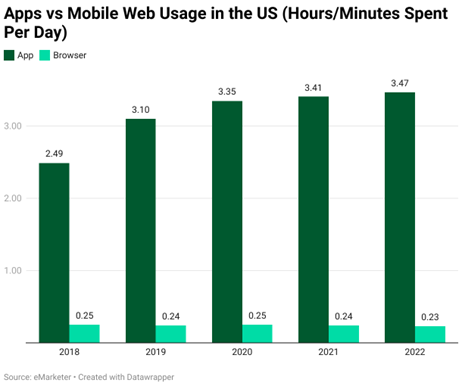
\includegraphics[width=0.7\textwidth]{poza3.png}
  \caption{Aplicații mobile vs. Web}
  \label{fig:mobile}
\end{figure}

\newpage
Câteva dintre caracteristicile principale pentru care utilizatorii preferă aplicațiile mobile în detrimentul celor web:
\begin{itemize}
        \item \textbf{Mai multe funcționalități} – o aplicație mobilă este capabilă să ofere un nivel mult mai ridicat de funcționalități față de site-urile web cum ar fi GPS-ul, camera, notificările și multe altele.
        \item \textbf {Viteză mai mare de rulare }– datorită faptului că acestea sunt descărcate direct pe telefonul mobil, pot fi accesate mult mai ușor față de cele web, astfel utilizatorii economisesc timp
        \item \textbf{Conexiune} – față de aplicațiile web care necesită conexiune la internet pentru a rula, aplicațiile mobile pot rula foarte ușor și când sunt offline datorită caracteristicilor pe care unele aplicații le dețin
        \item \textbf{Securitate}– aplicațiile mobile au mai multe protocoale de securitate ceea ce le fac mult mai sigure de utilizat
       
    \end{itemize}

În urma acestor avantaje pe care aplicațiile web le dețin, am decis să implementez o aplicație mobile în detrimentul unei simple pagini web. În cercetarea mea se află și câteva aplicații de la care a pornit ideea aplicației mele.
\subsubsection{Restograf}
Restograf    este o platformă dezvoltată pentru mai multe restaurante din România. Această aplicație a fost lansată în anul 2011, cu scopul de a facilita rezervarea unei mese. Prin această aplicație se poate face o rezervare într-un timp extrem de scurt, totodată se pot afla și lucruri pe care poate nu le știai despre restaurantele înscrise în aplicație sau poți să lași un feedback sau o părere despre mâncare, local și servire. Misiunea lor a fost să transforme rezervarea tradițională într-o rezervare simplă cu un răspuns rapid în timp real. Pe lângă rezervarea online, sunt și o mulțime de articole despre restaurante pe care e bine să le citești înainte să faci o rezervare la un anumit restaurant. Un model de rezervare este prezent in figura (\ref{fig:rezervare})

\begin{figure}[ht]
\centering
  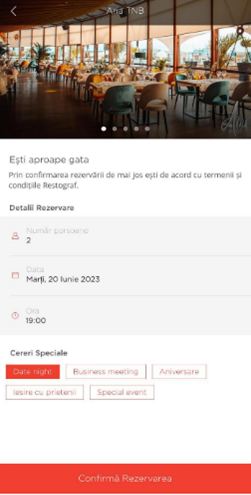
\includegraphics[width=0.3\textwidth]{poza4.png}
  \caption{Exemplu de rezervare}
  \label{fig:rezervare}
\end{figure}

\subsubsection{IALOC.Ro}
Ialoc  este atât o aplicație mobile cât șu un site web de rezervare a unei mese dintr-un restaurant. Această aplicație prezintă numeroase locații din diferite orașe ale României, unde poți lua masa. Totodată, dacă ești nehotărât la ce local ai vrea să mănânci, Ialoc vine în ajutor cu o mulțime de recomandări și topuri despre restaurantele din zonă. Deasemenea, în funcție de natura rezervării, ai posibilitatea să filtrezi restaurantele dupa bunul plac.

\subsubsection{Find a Table}
Find a Table  este o platformă online de rezervare a unei mese dintr-un restaurant. Aceasta a fost înființată în anul 2019 de către Alina Budai, CEO si Fondatorul platformei. Platforma deține și o rubrică de întrebări de la diferiți clienți cu diferite probleme întâmpinate pe platformă pentru diminuarea problemelor viitoare. 

\subsubsection{ZONIZ}
Zoniz  este o aplicație atât pentru clienții de restaurante cât și pentru ospătari. Prin această aplicație, clienții pot comanda direct din aplicație ce doresc să consume fără a mai fi nevoit ospătarul să preia comanda și să o noteze în carnețel. Totul este digitalizat, astfel ospătarii vor primi în format digital detaliile comenzii. Totodată, prin aplicația destinată ospătarilor, aceștia vor putea urmări demersul rezervării foarte rapid și eficient fără a mai fi nevoit să se deplaseze la masă. 
\subsubsection{Comparație sistem propus cu sistemele similare}
În acest subcapitol se vor evidenția funcționalitățile aplicațiilor găsite în comparație cu aplicația propusă. Criteriile de comparare vor fi operațiile de utilizator, administrarea contului, rezervări, asistență digitalizată. Comparatia se poate vedea in Tabelul (\ref{tab:tabel-comparatie})

\begin{table}[htb]
\caption{Comparatie intre sistemul propus si sisteme similare}
    \centering          % tabelul va fi centrat pe pagina
  \begin{tabular}{|l|c|c|c|c|c|c} % coloanele sunt separate cu linie verticala, prima e aliniata la stanga, restul centrate
    \hline
    \textbf{Functionalitate} & \textbf{Resograf} & \textbf{IALOC} & \textbf{Find a Table} & \textbf{Zoniz} & \textbf{SP} \\ 
    \hline % aici s-a introdus o linie orizontala
    \hspace*{\fill} Modul operatii utilizator  \hspace*{\fill}
    \\
    \hline
    Autentificare & DA & DA & DA & DA & DA  \\
    \hline
   Inregistrare folosind FB & DA & DA & DA & DA & NU \\
   \hline
   Inregistrare folosind GG & DA & DA & DA & DA & DA \\
    \hline
    Inregistrare email & DA & DA & DA & DA & DA \\
    \hline
    Delogare & DA & DA & DA & DA & DA \\
    \hline
  \end{tabular}
  \label{tab:tabel-comparatie}
\end{table}
\chapter{Analiza, Proiectare, Implementare}

\section{Analiză și Proiectare }
Acest subcapitol va detalia arhitectura aplicației prin detalierea fiecărei diagrame realizate. Pe lângă acestea, se vor prezenta și tehnologiile folosite, atât pentru componenta de backend cât și pentru componenta de frontend.  
\subsection{Arhitectura sistemului}
În cadrul acestui subcapitol se vor detalia diagramele realizate specific pentru aplicația propusă.
\subsubsection{Diagrama conceptuală a sistemului}
Diagrama conceptuală a sistemului urmărește legătura dintre componentele 
necesare și buna funcționare a aplicației. Atât userul cât și adminul se vor putea 
conecta la aplicația Android prin intermediul internetului, cu ajutorul căruia se va accesa 
baza de date online Firebase.\cite{aplication}
Adminul va avea acces la toate informațiile stocate în baza de date Firebase, cum ar 
fi detaliile utilizatorilor înscriși, programările efectuate de aceștia, locația și meniul 
restaurantului, informații care pot fi modificate ulterior de acesta.
Cât despre user, acesta are acces doar la informațiile stocate în baza de date 
referitoare la propriile rezervări și datele de contact pe care le poate și modifica. Cu ajutorul ecuatiei (\ref{ecuatie1}) se poate calcula diagrama conceptuala.

\begin{equation}
  \begin{cases}
    x + y = 5 \\
    2x - y = 1
  \end{cases}
  \label{ecuatie1}
\end{equation}
\subsubsection{Arhitectura aplicației ANDROID}
Arhitectura sistemuluui de operare Android este o arhitectură layered. 
Cel mai de jos strat în ierarhia arhitecturii este stratul HTTP care primește și 
trimite cereri HTTP către server. Stratul API analizază răspunsul de la server și îl 
formulează sub formă de interogare pentru a-l putea trimite sub formă de string către 
stratul superior. Implementarea funcțiilor necesare este inclusă în stratul Generic Data. 
Aceasta arhitectura se obtine cu ajutorul ecuatiei (\ref{ecuatie1}).
\begin{equation}
    \centering
  \label{ecuatie2}
  f(x) = x^2 + 2x + 1
\end{equation}
\section{Implementare}
În acest subcapitol, se va prezenta modul de utilizare al aplicației prin trecerea în revistă a mai multor aspecte precum cerințele sistemului, descrierea cazurilor de utilizare pentru cei doi actori ai proiectului (admin și user) și totdată descrierea unui manual de utilizare al aplicației.
\subsection{Modul de implementare al aplicatiei}
În următoarea parte va fi prezent modul de utilizare al aplicației din perspectiva 
adminului și din perspectiva userului.
Prima pagină este o pagină comună pentru cele două tipuri de utilizatori, 
reprezentând pagina de pornire a aplicației. În ea se regăsesc 2 butoane, care reprezintă 
următorul pas spre intrarea în aplicație. Există butonul de Login prin care se pot 
autentifica utilizatorii deja existenți în baza de date a aplicației și adminul care nu are 
nevoie de înregistrare deoarece acesta face parte din administrația aplicației și butonul 
de Register prin care utilizatorii noi veniți își pot crea cont în cadrul aplicației. Această 
pagină se regăsește în Figură (\ref{fig:welcome}) după cum urmează :

\begin{figure}[ht]
\centering
  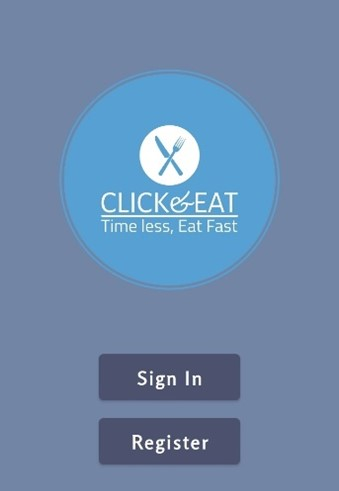
\includegraphics[width=0.2\textwidth]{poza5.jpg}
  \caption{Pagina de Welcome}
  \label{fig:welcome}
\end{figure}

\subsubsection{Aplicația din perspectiva utilizatorului cu rolul de admin}
La prima accesare a aplicației la apăsarea butonului de Sign In din cadrul activității de Welcome , utilizatorul este direcționat către activitatea de Login  pentru a se putea loga. Acesta nu are nevoie de înregistrare în aplicație precum utilizatorii cu rol de user deoarece face parte din administrația restaurantului, credențialele fiind special create pentru acesta. În cazul în care s-a conectat recent în aplicație, acesta rămâne conectat, iar la apăsarea butonului de Sign In, va fi direct direcționat către activitatea de AdminHome din cadrul aplicației.
Una dintre cerintele functionale \cite{city} este prezentatat in tabelul (\ref{tab:tabel-cerinte})

\begin{table}[htb]
\caption{Descrierea cerințelor funcționale ale aplicației}

    \centering          % tabelul va fi centrat pe pagina
  \begin{tabular}{|l|c|c|} % coloanele sunt separate cu linie verticala, prima e aliniata la stanga, restul centrate
    \hline
    \textbf{Cerinta functionala} & \textbf{Utilizator}  \\ 
    \hline % aici s-a introdus o linie orizontala
    Autentificare & Admin, User  \\
    \hline
   Inregistrare & User  \\
   \hline
   Delogare & Admin, User  \\
    \hline
    Stergere cont admininstrator & Admin  \\
    \hline
     Stergere cont user & User   \\
    \hline
  \end{tabular}
  \label{tab:tabel-cerinte}
\end{table}
În urma procesului de alegere a mesei, utilizatorul va fi direcționat spre pagina cu rezervarea propriu-zisă. În cadrul acelei pagini, userul va mai avea câteva lucruri de ales înainte de finalizarea rezervării. Mai exact va trebui să aleagă data în care va dori să fie rezervare, ora la care va avea loc cât și detalii despre persoana de contact cu mar fi adresa de e-mail și numele. În urma procesului de selectare a informațiilor, se va verifica cu baza de date dacă este liberă data și ora pentru masa respectivă. În cazul în care răspunsul este unul afirmativ, rezervarea va avea loc iar utilizatorului i se va trimite un e-mail de confirmare cu toate datele aferente procesului de rezervare. Dacă răspunsul este unul negativ, se va afișa un mesaj prin care anunță userul că masa este deja ocupată și să aleagă o altă masă sau dată pentru rezervarea sa. 


\printbibliography[heading=bibintoc]

\end{document}
